\documentclass[10pt,a4paper]{article}
\usepackage{amsmath,amssymb,amsthm,graphicx}
% Independent article wrapper; no publisher class or third-party style redistribution.
\usepackage[margin=25mm]{geometry}
\usepackage{fontspec}
\setmainfont{Latin Modern Roman}
\usepackage{amsmath,amssymb,amsthm,mathtools,graphicx}
\usepackage{hyperref}
\hypersetup{hidelinks}
\newtheorem{cdrthm}{Theorem}[section]
\newtheorem{theo}[cdrthm]{Theorem}
\newtheorem{prop}[cdrthm]{Proposition}
\newtheorem{lemm}[cdrthm]{Lemma}
\newtheorem{lemma}[cdrthm]{Lemma}
\newtheorem{coro}[cdrthm]{Corollary}
\theoremstyle{definition}
\newtheorem{defi}[cdrthm]{Definition}
\theoremstyle{remark}
\newtheorem{rema}[cdrthm]{Remark}

\usepackage{tikz}
\usepackage[all]{xy}
\newtheorem{exam}[cdrthm]{Example}
\newtheorem{nota}[cdrthm]{Notation}

% Native author section 5 macros, published.tex lines 1879--1889
\newcommand{\cpA}{\cup \Ab}
\newcommand{\prA}{\times \Ab}
\newcommand{\Cgeo}{C}
\newcommand{\susst}{\subseteq^*}
\newcommand{\Ctbu}{\tilde{C}_{\bullet}}
\newcommand{\Ctalg}{\tilde{{\mathcal C}}_{\bullet}}
\newcommand{\Ctcal}{\tilde{{\mathcal C}}}
\newcommand{\Calg}{{\mathcal C}_{\bullet}}
\newcommand{\Falg}{{\mathcal F}_{\bullet}}
\newcommand{\Fal}{{\mathcal F}}
\newcommand{\Cal}{{\mathcal C}}
% Original author macros, published lines 70--437 and 1563--1564.
\theoremstyle{plain}
\newtheorem{problem}{Problem}
\newtheorem{fact}{Fact}

\newcommand{\psp}[1]{{{\bf P}^{#1}}}
\newcommand{\psr}[1]{{\bf P}(#1)}

\newcommand{\ini}[1]{\text{in}(#1)}
\newcommand{\gin}[1]{\text{gin}(#1)}
\newcommand{\kr}{{\Bbbk}}
\newcommand{\pd}{\partial}
\newcommand{\vardel}{\partial}
\renewcommand{\tt}{{\bf t}}



\newcommand{\coh}{{{\text{{\rm coh}}}}}

\newcommand{\modv}[1]{{#1}\text{-{mod}}}
\newcommand{\modstab}[1]{{#1}-\underline{\text{mod}}}


\newcommand{\sut}{{}^{\tau}}
\newcommand{\sumit}{{}^{-\tau}}
\newcommand{\til}{\thicksim}


\newcommand{\totp}{\text{Tot}^{\prod}}
\newcommand{\dsum}{\bigoplus}
\newcommand{\dprod}{\prod}
\newcommand{\lsum}{\oplus}
\newcommand{\lprod}{\Pi}

\newcommand{\La}{{\Lambda}}

\newcommand{\sirstj}{\circledast}

\newcommand{\she}{\EuScript{S}\text{h}}
\newcommand{\cm}{\EuScript{CM}}
\newcommand{\cmd}{\EuScript{CM}^\dagger}
\newcommand{\cmri}{\EuScript{CM}^\circ}
\newcommand{\cler}{\EuScript{CL}}
\newcommand{\clerd}{\EuScript{CL}^\dagger}
\newcommand{\clerri}{\EuScript{CL}^\circ}
\newcommand{\gor}{\EuScript{G}}
\newcommand{\cF}{\mathcal{F}}
\newcommand{\cG}{\mathcal{G}}

\newcommand{\cM}{\mathcal{M}}
\newcommand{\cE}{\mathcal{E}}

\newcommand{\cI}{\mathcal{I}}
\newcommand{\cP}{\mathcal{P}}
\newcommand{\cK}{\mathcal{K}}

\newcommand{\cS}{\mathcal{S}}
\newcommand{\cC}{\mathcal{C}}
\newcommand{\cO}{\mathcal{O}}
\newcommand{\cJ}{\mathcal{J}}
\newcommand{\cU}{\mathcal{U}}

\newcommand{\cQ}{\mathcal{Q}}
\newcommand{\cX}{\mathcal{X}}
\newcommand{\cY}{\mathcal{Y}}
\newcommand{\cZ}{\mathcal{Z}}
\newcommand{\cV}{\mathcal{V}}

\newcommand{\mm}{\mathfrak{m}}

\newcommand{\dlim} {\varinjlim}
\newcommand{\ilim} {\varprojlim}


\newcommand{\CM}{\text{CM}}
\newcommand{\Mon}{\text{Mon}}

\newcommand{\Kom}{\text{Kom}}

\newcommand{\EH}{{\mathbf H}}
\newcommand{\res}{\text{res}}
\newcommand{\Hom}{{\rm{Hom}}}
\newcommand{\inhom}{{\underline{\text{Hom}}}}
\newcommand{\Ext}{\text{Ext}}
\newcommand{\Tor}{\text{Tor}}
\newcommand{\ghom}{\mathcal{H}om}
\newcommand{\gext}{\mathcal{E}xt}
\newcommand{\id}{\text{{id}}}
\newcommand{\im}{\text{im}\,}
\newcommand{\codim} {\text{codim}\,}
\newcommand{\resol}{\text{resol}\,}
\newcommand{\rank}{\text{rank}\,}
\newcommand{\lpd}{\text{lpd}\,}
\newcommand{\coker}{\text{coker}\,}
\newcommand{\supp}{\text{supp}\,}
\newcommand{\Ad}{A_\cdot}
\newcommand{\Bd}{B_\cdot}
\newcommand{\Fd}{F_\cdot}
\newcommand{\Gd}{G_\cdot}

\newcommand{\sus}{\subseteq}
\newcommand{\sups}{\supseteq}
\newcommand{\pil}{\rightarrow}
\newcommand{\vpil}{\leftarrow}
\newcommand{\rpil}{\leftarrow}
\newcommand{\lpil}{\longrightarrow}
\newcommand{\inpil}{\hookrightarrow}
\newcommand{\pils}{\twoheadrightarrow}
\newcommand{\projpil}{\dashrightarrow}
\newcommand{\dotpil}{\dashrightarrow}
\newcommand{\adj}[2]{\overset{#1}{\underset{#2}{\rightleftarrows}}}
\newcommand{\mto}[1]{\stackrel{#1}\longrightarrow}
\newcommand{\vmto}[1]{\stackrel{#1}\longleftarrow}
\newcommand{\mtoelm}[1]{\stackrel{#1}\mapsto}
\newcommand{\bihom}[2]{\overset{#1}{\underset{#2}{\rightleftarrows}}}
\newcommand{\eqv}{\Leftrightarrow}
\newcommand{\impl}{\Rightarrow}

\newcommand{\iso}{\cong}
\newcommand{\te}{\otimes}
\newcommand{\into}[1]{\hookrightarrow{#1}}
\newcommand{\ekv}{\Leftrightarrow}
\newcommand{\equi}{\simeq}
\newcommand{\isopil}{\overset{\cong}{\lpil}}
\newcommand{\equipil}{\overset{\equi}{\lpil}}
\newcommand{\ispil}{\isopil}
\newcommand{\vvi}{\langle}
\newcommand{\hvi}{\rangle}
\newcommand{\susneq}{\subsetneq}
\newcommand{\sgn}{\text{sign}}


\newcommand{\xd}{\check{x}}
\newcommand{\ortog}{\bot}
\newcommand{\tL}{\tilde{L}}
\newcommand{\tM}{\tilde{M}}
\newcommand{\tH}{\tilde{H}}
\newcommand{\tvH}{\widetilde{H}}
\newcommand{\tvh}{\widetilde{h}}
\newcommand{\tV}{\tilde{V}}
\newcommand{\tS}{\tilde{S}}
\newcommand{\tT}{\tilde{T}}
\newcommand{\tR}{\tilde{R}}
\newcommand{\tf}{\tilde{f}}
\newcommand{\ts}{\tilde{s}}
\newcommand{\tp}{\tilde{p}}
\newcommand{\tr}{\tilde{r}}
\newcommand{\tfst}{\tilde{f}_*}
\newcommand{\empt}{\emptyset}
\newcommand{\bfa}{{\mathbf a}}
\newcommand{\bfb}{{\mathbf b}}
\newcommand{\bfd}{{\mathbf d}}
\newcommand{\bfl}{{\mathbf \ell}}
\newcommand{\bfx}{{\mathbf x}}
\newcommand{\bfm}{{\mathbf m}}
\newcommand{\bfv}{{\mathbf v}}
\newcommand{\bft}{{\mathbf t}}
\newcommand{\bbfa}{{\mathbf a}^\prime}
\newcommand{\la}{\lambda}
\newcommand{\bfen}{{\mathbf 1}}
\newcommand{\bfe}{{\mathbf 1}}
\newcommand{\ep}{\epsilon}
\newcommand{\en}{r}
\newcommand{\tu}{s}
\newcommand{\Sym}{\text{Sym}}

\newcommand{\ome}{\omega_E}

\newcommand{\bevis}{{\bf Proof. }}
\newcommand{\demofin}{\qed \vskip 3.5mm}
\newcommand{\nyp}[1]{\noindent {\bf (#1)}}
\newcommand{\demo}{{\it Proof. }}
\newcommand{\demodone}{\demofin}
\newcommand{\parg}{{\vskip 2mm \addtocounter{theorem}{1}  
                   \noindent {\bf \thetheorem .} \hskip 1.5mm }}

\newcommand{\lcm}{{\text{lcm}}}

\newcommand{\dl}{\Delta}
\newcommand{\cdel}{{C\Delta}}
\newcommand{\cdelp}{{C\Delta^{\prime}}}
\newcommand{\dlst}{\Delta^*}
\newcommand{\Sdl}{{\mathcal S}_{\dl}}
\newcommand{\lk}{\text{lk}}
\newcommand{\lkd}{\lk_\Delta}
\newcommand{\lkp}[2]{\lk_{#1} {#2}}
\newcommand{\del}{\Delta}
\newcommand{\delr}{\Delta_{-R}}
\newcommand{\dd}{{\dim \del}}
\newcommand{\Del}{\Delta}

\newcommand{\bb}{{\mathbf b}}
\newcommand{\cc}{{\mathbf c}}
\newcommand{\xx}{{\mathbf x}}
\newcommand{\yy}{{\mathbf y}}
\newcommand{\zz}{{\mathbf z}}
\newcommand{\mv}{{\xx^{\aa_v}}}
\newcommand{\mF}{{\xx^{\aa_F}}}

\newcommand{\Symm}{\text{Sym}}
\newcommand{\pnm}{{\mathbf P}^{n-1}}
\newcommand{\opnm}{{\go_{\pnm}}}
\newcommand{\ompnm}{\omega_{\pnm}}

\newcommand{\pn}{{\mathbf P}^n}
\newcommand{\hele}{{\mathbb Z}}
\newcommand{\nat}{{\mathbb N}}
\newcommand{\rasj}{{\mathbb Q}}
\newcommand{\bfone}{{\mathbf 1}}

\newcommand{\dt}{\bullet}

\newcommand{\disk}{\scriptscriptstyle{\bullet}}

\newcommand{\cxF}{F_\dt}
\newcommand{\pol}{f}

\newcommand{\Rn}{{\mathbb R}^n}
\newcommand{\An}{{\mathbb A}^n}
\newcommand{\frg}{\mathfrak{g}}
\newcommand{\PW}{{\mathbb P}(W)}

\newcommand{\pos}{{\mathcal Pos}}
\newcommand{\g}{{\gamma}}

\newcommand{\Vaa}{V_0}
\newcommand{\Bp}{B^\prime}
\newcommand{\Bpp}{B^{\prime \prime}}
\newcommand{\bbp}{\mathbf{b}^\prime}
\newcommand{\bbpp}{\mathbf{b}^{\prime \prime}}
\newcommand{\bp}{{b}^\prime}
\newcommand{\bpp}{{b}^{\prime \prime}}

\newcommand{\oLa}{\overline{\Lambda}}
\newcommand{\ov}[1]{\overline{#1}}
\newcommand{\ovv}[1]{\overline{\overline{#1}}}
\newcommand{\tm}{\tilde{m}}
\newcommand{\po}{\bullet}

\newcommand{\surj}[1]{\overset{#1}{\twoheadrightarrow}}
\newcommand{\Supp}{\text{Supp}}

\newcommand{\ZZ}{{\mathbb Z}}
\newcommand{\NN}{{\mathbb N}}
\newcommand{\RR}{{\mathbb R}}

\newcommand{\oR}{\overline{R}}

\newcommand{\bfu}{{\mathbf u}}
\newcommand{\nn}{{\mathbf n}}
\newcommand{\oa}{\overline{a}}
\newcommand{\cop}{\text{cop}}

\newcommand{\opos}{\text{op}\,}

\newcommand{\ngmi}{\text{neg}}
\newcommand{\up}{\text{up}}
\newcommand{\dw}{\text{down}}

\newcommand{\diw}[1]{\widehat{#1}}
\newcommand{\di}[1]{\diw{#1}}
\newcommand{\bo}{b}
\newcommand{\ub}{u}
\newcommand{\fs}{\infty}
\newcommand{\ifst}{\infty}
\newcommand{\mon}{{mon}}
\newcommand{\cl}{\text{cl}}
\newcommand{\intr}{\text{int}}
\newcommand{\ul}[1]{\underline{#1}}

\newcommand{\bipil}{\leftrightarrow}
\newcommand{\bfc}{{\mathbf c}}

\renewcommand{\mp}{m^\prime}

\newcommand{\np}{n^\prime}
\newcommand{\Mod}{\text{Mod }}
\newcommand{\Sh}{\text{Sh } }
\newcommand{\st}{\text{st}}

\newcommand{\hM}{\tilde{M}}
\newcommand{\hs}{\tilde{s}}
\newcommand{\ee}{\mathbf{e}}

\newcommand{\lex}{{\text{lex}}}
\newcommand{\ordGL}{\succeq_{\lex}}
\newcommand{\ordG}{\succ_{\lex}}
\newcommand{\ordML}{\preceq_{\lex}}
\newcommand{\ordM}{\prec_{\lex}}
\newcommand{\tLa}{\tilde{\Lambda}}
\newcommand{\tGa}{\tilde{\Gamma}}
\newcommand{\STS}{\text{STS}}
\newcommand{\ii}{{\rotatebox[origin=c]{180}{\scalebox{0.7}{\rm{!}}}}}

\newcommand{\jj}{\mathbf{j}}

\newcommand{\shmod}{\texttt{shmod}\,}
\newcommand{\hf}{\underline{f}}
\newcommand{\Glim}{\lim}
\newcommand{\Gcolim}{\colim}
\newcommand{\fm}{f^{\underline{m}}}
\newcommand{\fn}{f^{\underline{n}}}
\newcommand{\gn}{g_{\mathbf{|}n}}
\newcommand{\se}[1]{\overline{#1}}
\newcommand{\cB}{{\mathcal{B}}}
\newcommand{\fin}{{\text{fin}}}
\newcommand{\Poset}{{\text{\bf Poset}}}
\newcommand{\Set}{{\text{\bf Set}}}

\newcommand{\Homi}{\text{Hom}^{L}}
\newcommand{\Homb}{\text{Hom}_S}
\newcommand{\Homu}{\text{Hom}^u}
\newcommand{\bfnu}{{\mathbf 0}}

\newcommand{\semip}{up semi-finite }
\newcommand{\semim}{down semi-finite }
\newcommand{\dif}[1]{\di{#1}_{fin}}
\newcommand{\llin}{\raisebox{1pt}{\scalebox{1}[0.6]{$\mid$}}}
\newcommand{\promap}{\mathrlap{{\hskip 2.8mm}{\llin}}{\lpil}}
\newcommand{\dual}{{\widehat{}}}
\newcommand{\Bool}{{\bf Bool }}
\newcommand{\pro}{{pro}}
\newcommand{\ovF}{\overline{F}}
\newcommand{\TO}{{\mathrm to}}
\newcommand{\dT}{\overset{\rightarrow}{T}}

\newlength{\dhatheight}
\newcommand{\doublehat}[1]{
    \settoheight{\dhatheight}{\ensuremath{\widehat{#1}}}
    \addtolength{\dhatheight}{-0.35ex}
    \widehat{\vphantom{\rule{1pt}{\dhatheight}}
    \smash{\widehat{#1}}}}

\newcommand{\napo}{natural }

\newcommand{\colim}{\text{colim}}
\newcommand{\oPsi}{\overline{\Psi}}
\newcommand{\bfC}{{\mathbf C}}
\newcommand{\bfi}{{\mathbf i}}
\newcommand{\ik}{{\mathfrak k}}
\newcommand{\ic}{{\mathfrak c}}

\newcommand{\ijfr}{{\mathfrak j}}
\newcommand{\iifr}{{\mathfrak i}}

\newcommand{\iC}{{\mathfrak C}}

\newcommand{\Ab}{A_\bullet}
\newcommand{\Rb}{R_\bullet}
\newcommand{\oDo}{\overline{D^\opos}}
\newcommand{\bfA}{{\mathbf A}}
\newcommand{\het}{\text{ht}}

\newcommand{\bfal}{{\mathbf{ \alpha}}}
\newcommand{\al}{{\alpha}}
\newcommand{\alp}{{\alpha^\prime}}
\newcommand{\tci}{tight}
\newcommand{\bitci}{bitight}
\newcommand{\oD}{\overline{D}}
\newcommand{\Delst}{\vardel \Delta}
\newcommand{\mlin}{-}

\newcommand{\ben}{{\mathbf 1}}
\newcommand{\bfj}{{\mathbf j}}
\newcommand{\bfio}{\hat{\bfi}}
\newcommand{\pot}{{\rm{pos}}}
\newcommand{\rac}{r-acyclic}

\newcommand{\Ign}[1]{}
\newcommand{\bfr}{{\mathbf r}}
\newcommand{\bfq}{{\mathbf q}}
\title{The saturated rainbow cell complex resolves precisely the rainbow ideals with linear resolution}
\author{Gunnar Fløystad, Ine Gabrielsen, Amir Mafi}
\date{doi:10.5802/alco.500; CC BY 4.0}
\begin{document}
\maketitle
\noindent\textit{Editorial note.} Exact corrected published version only.\par\medskip
\noindent\textit{Editorial note.} Original author text and native diagrams retained; only counter and wrapper presentation additions.\par\medskip
\noindent\textit{Editorial note.} Unchanged macros, official bibliography and license evidence reused by explicit paths from ALCO500.\par\medskip
\noindent\textit{Editorial note.} r002 restores unchanged native section 5 macros from official published.tex lines 1879–1889; r001 failed on missing susst. No author mathematical text changed.\par\medskip
\noindent\textit{Editorial scope.} Faithful author material collection only. Root owns assembly, compile, visual QA, SQLite, upload and identity refresh.\par\medskip
\noindent\textit{Allowed standard prerequisites (editorial).}\begin{itemize}
\item Labelled cellular complexes and multigraded homology. Miller–Sturmfels, Combinatorial commutative algebra, published reference [39], Section 4 (MiSt). Standard construction and degree-strand identification, explicitly stated in full as Fact 1.
\item Minimal multigraded free resolutions, comparison-map lifting and homology exact sequences. Standard homological algebra over the polynomial ring k[A]. Lifting identity to a homogeneous chain map and the exact homology sequence; the degree-controlled comparison and cokernel induction are current author core and retained in full.
\end{itemize}\medskip
\section*{Source and counting boundary}
Gunnar Fløystad, Ine Gabrielsen and Amir Mafi, \emph{Polarizations of Artin monomial ideals}, Algebraic Combinatorics 9(4) (2026), 993--1035, \url{https://doi.org/10.5802/alco.500}. Official published article content and native mathematical TeX are licensed CC BY 4.0, \url{https://creativecommons.org/licenses/by/4.0/}; copyright remains with the authors.

Only whole Theorem 5.5 (\texttt{thm:cell-linres}) is counted. Its full current support, particularly Proposition 5.4, is retained but not separately counted. This is independent of the ball/constructibility Theorem 4.3 collected separately: neither proof uses the other. Remark 5.6 and subsequent corollaries are omitted.

\paragraph{Version boundary.} The earlier arXiv:2212.09528v2 was withdrawn on 5 August 2024 because of the authors' stated error in old Lemma 6.17, 1a, Case iii, affecting old Theorem 6.7. The v3 announcement on 13 January 2025 states the error was fixed. Only the actual corrected 2026 official published text is used here. No withdrawn bitight-equivalence argument, version mixing, mathematical repair or certification is supplied. Notices: \url{https://arxiv.org/abs/2212.09528v2}, \url{https://arxiv.org/abs/2212.09528v3}.

\paragraph{Presentation.} Native author mathematical text and macros are preserved. An independent article wrapper and explicit counter settings restore published numbering. The square figure is retained as native TikZ and the comparison diagram as native xymatrix; no external image is required. The complete official bibliography is reused with original numbers and citation keys. Publisher classes, logos and third-party styles are excluded.

\paragraph{Difficulty and scope.} The H2 core is the saturation argument giving the homology gap $p+n+2$, followed by degree-controlled comparison-map and cokernel induction. Miller--Sturmfels [39], Section 4, is standard external background; the current author core is reproduced fully. Saved in-flight identity information ends on 14 October 2026 at 17:36:45 UTC; later overlap remains unconfirmed. This is author-material preparation, not mathematical certification or final global-unique admission.

\setcounter{section}{3}\setcounter{equation}{3}

Let  $A_1, A_2, \ldots, A_n$ be disjoint finite sets, and $A = \sqcup_{i=1}^n A_i$
their union. The complete intersection ideal
\begin{equation*}
  C = (m(A_1), m(A_2), \ldots, m(A_n))  \sus k[A]
\end{equation*}
is the SR-ideal of the join
of the boundaries of simplices
\begin{equation} \label{eq:liaison-join}
  \Delst(\Ab) = \pd \Delta(A_1) * \pd \Delta(A_2) * \cdots * \pd \Delta(A_n),
 \end{equation}

\setcounter{subsection}{1}

\subsection{Rainbow ideals}
Denote $\bfA = A_1 \times A_2 \times \cdots \times A_n$.
For $\bfa = (a_1, a_2, \ldots, a_n)$ in $\bfA$, denote
by $[\bfa ]$ the set $\{a_1, a_2, \ldots, a_n \}$. 

\setcounter{cdrthm}{1}

For $\bfa \in \bfA$ let $m(\bfa)$ be the monomial 
$\prod_{i = 1}^n a_i$. Thinking
of $A_i$ as a color class, we call such a monomial a {\it rainbow
monomial}.  The Alexander dual ideal $B$ of the complete intersection
$C = (m(A_1), \ldots, m(A_n))$ is generated by the complements
of the facets of $\Delst(\Ab)$, and so it is the monomial
ideal generated by all the  rainbow monomials. Letting
$(A_i)$ be the ``color ideal'' generated by the elements of $A_i$ (considered
as variables), then $B$ is the product of these color ideals:
\[ B  = (m(\bfa) \, | \, \bfa \in \bfA) = \prod_{i = 1}^n(A_i). \]

\begin{defi}
For a subset $T \sus \bfA$, denote by $I(T)$ the ideal generated
by $m(\bfa)$ for $\bfa \in T$. Such an ideal is called a {\it rainbow ideal}.
For the complement set $T^c = \bfA \backslash T$, we
usually write $L(T)$ for $I(T^c)$, the {\it complement} rainbow ideal.
\end{defi}

\setcounter{section}{5}\setcounter{subsection}{1}\setcounter{cdrthm}{0}\setcounter{equation}{6}\setcounter{figure}{5}

A finite set $A$ gives rise to the geometric
simplex spanned by the elements of $A$:
\[ \Delta(A) = \left\{\sum_{a \in A} \gamma_a \cdot a \, | \, 0 \leq \gamma_a \leq 1,  \sum_{a \in A} \gamma_a = 1 \right\} \sus \RR^A. \]
Given finite non-empty sets $ A_1, A_2, \ldots, A_n$, 
we get a polytope: 
\[ \Pi(\Ab) = \Delta(A_1) \times \Delta(A_2) \times \cdots
\times \Delta(A_n) \sus \times_{i = 1}^n \RR^{A_i} = \RR^A. \]
Its dual (or polar) polytope
is the join
\[ \Delst(\Ab) =  \pd \Delta(A_1) * \pd \Delta(A_2) * \cdots * \pd \Delta(A_n).
\]
The set of vertices of $\Pi(\Ab)$ is the set $A_1 \times \cdots \times
A_n$.

\begin{nota}
  When  $R_i \sus A_i$ for $ i = 1, \ldots, n$ are {\it non-empty} subsets,
  we write $\Rb \susst \Ab$.
\end{nota}


\begin{defi}
  The polytope $\Pi(\Ab)$ gives rise to a cell complex $\Cgeo(\Ab)$,
  actually a polyhedral cell complex,
whose cells are the $\Pi(\Rb)$ with $\Rb \susst \Ab$. 
The dimension of such a cell is $\sum_i |R_i| - n$.
A subset $T \sus A_1 \times A_2 \times \cdots \times A_n$
induces a cell subcomplex $C(T)$ of $\Cgeo(\Ab)$ consisting of all
$\Pi(\Rb)$ such
$R_1 \times R_2 \times \cdots \times R_n \sus T$.
We say $C(T)$ is the {\it saturated} cell sub-complex of
$\Cgeo(\Ab)$ associated to $T$. 
\end{defi}

\medskip
\noindent{{\bf The (augmented) chain complex:}}
\begin{equation} \label{eq:minfree-Ct}
  \Ctbu(T): C_{-1}(T) \vpil C_0(T) \vpil C_1(T) \vpil
  \cdots \vpil C_p(T) \vpil \cdots ,
\end{equation}
where $C_p(T)$ is the $k$-vector space with basis all cells
of $\Cgeo(T)$ of dimension $p$ (and $C_{-1}(T)$ is the one-dimensional
vector space with basis the empty cell), and standard differentials
(see~\eqref{eq:minfree-diff} below). The homology groups are the
reduced homology groups. Note that $\tilde{H}_{-1}(\Ctbu(T)) \neq 0$ iff
$T$ is empty. 

Let $S$ be the polynomial ring $k[A]$ whose variables
are the elements of $A = A_1 \cup \cdots \cup A_n$. 
A vertex $\bfa = (a_1,a_2, \ldots, a_n)$ of $\Pi(\Ab)$
may be labelled by the monomial
$m(\bfa) = a_1a_2\cdots a_n$. The cell $\Pi(\Rb)$ is then labelled by
the least common multiple of the monomials on its vertices. This is
simply
\[ m(\Rb) = m(R_1)m(R_2) \cdots m(R_n), \text{ where }
  m(R_i) = \prod_{r \in R_i}r,\]
which is a monomial of degree $\dim \Pi(\Rb) + n$. 

\medskip
\noindent{\bf The (augmented) free cellular complex:}
  For $T \sus A_1 \times \cdots \times A_n$, this induces a labelling
by monomials of the cell sub-complex $\Cgeo(T)$.
By~\cite[Section 4]{MiSt} it then gives a {\it free cellular complex}
\[ \Ctalg(T) : \Cal_{-1}(T) \vmto{d_0} \Cal_0(T) \vmto{d_1}
  \cdots \vpil \Cal_p(T) \vpil \cdots , \]
where
$\Cal_p(T)$ is the free $S$-modules with generators all cells $\Pi(\Rb)$ in
$\Cgeo(T)$ of dimension $p$ (and $\Cal_{-1}(T) = S$).
The image of $d_0$ is $I(T)$.
We may put a total order on each $A_i$. Together with the ordered
sequence $A_1, A_2, \ldots, A_n$, this gives a total order on the
union $A = \cup_1^n A_i$. Then $\Rb \sus^{*} \Ab$ inherits a total order on
$R = \cup_1^n R_i$. For $b \in R$ denote by $\pot(b)$ its position in
this total order. For $p \geq 1$
the differential $d^p$ is then given by
\begin{equation} \label{eq:minfree-diff}
  \Pi(\Rb) \mapsto \sum_{\begin{matrix} i = 1, \ldots, n\\
      b \in R_i, |R_i| \geq 2 \end{matrix}}  (-1)^{\pot(b)} b \cdot
  \Pi(R_1, \ldots, R_i\backslash \{b \}, \ldots, R_n).
\end{equation}

\begin{exam} Let $A_1 = \{a_1, b_1\}$ and $A_2 = \{ a_2,b_2\}$ and
  $T = A_1 \times A_2$. The product polytope $\Pi (\Ab)$ is the
  square labelled as in Figure~\ref{fig:cell-square}.

\begin{figure}[ht]
\begin{center}

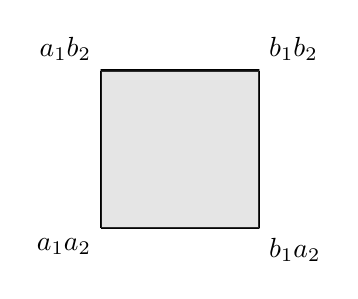
\begin{tikzpicture}[thick,scale=2]

\coordinate[label=-135:{$a_1a_2$}] (A1) at (0,0);
\coordinate[label=135:{$a_1b_2$}] (A2) at (0,1);
\coordinate[label=45:{$b_1b_2$}] (A3) at (1,1);
\coordinate[label=-45:{$b_1a_2$}] (A4) at (1,0);


\draw (A1) edge[] (A2); 
\draw (A2) edge[] (A3); 
\draw (A4) edge[swap] (A3); 
\draw (A1) edge[swap] (A4); 


\draw[fill=lightgray, opacity=0.4] (A1)--(A2)--(A3)--(A4)--(A1);

\end{tikzpicture}

\end{center}
\caption{The square $\Pi(\Ab)$, with monomial labels on vertices}
\label{fig:cell-square}
\end{figure}
  The augmented chain complex is
  \[ k \vpil k^4 \vpil k^4 \vpil k, \]
  which has no homology, it is acyclic.
  Let $S = k[a_1,b_1, a_2, b_2]$. The rainbow ideal is
  $I(T) = (a_1a_2, a_1b_2, b_1a_2, b_1b_2)$. The augmented  free cellular complex is
  \[ S \overset{d}{\vpil} S(-2)^4 \vpil S(-3)^4 \vpil S(-4). \]
  The image of $d$ is $I(T)$, and in this case,
  omitting the first term,  the complex is a minimal free resolution of $I(T)$. 
In general, if $T$ is the full $A_1 \times \cdots \times A_n$, the free cellular
complex is always a minimal free resolution of $I(T)$. Finding out for
which $T$ this free cellular
complex {\it is} a resolution, Theorem~\ref{thm:cell-linres},
is an aspect of the main result of our article. 
\end{exam}

\setcounter{fact}{0}

The generators of $\Cal_p(T)$ for $p \geq 0$ have degrees $p+n$,
so $\Ctcal_{\geq 0}(T)$ is a {\it linear}
free cellular complex.
The free cellular complex $\Ctalg(T)$ is $\NN^A$-graded. A family of subsets
$\Rb \susst \Ab$ gives a restriction
$T_{|R} = T \cap (R_1 \times \cdots \times R_n)$. 
It also gives a squarefree degree $\deg(\Rb) \in \NN^A$.
The free cellular complex  $\Ctalg(T)_{|\deg(\Rb)}$ in this specific degree
identifies as the augmented chain complex $\Ctbu(T_{|\Rb})$
(see~\eqref{eq:minfree-Ct}).

\begin{fact} \label{fact:cell-hom} Let $\Rb \sus^* \Ab$. 
  The homology of the augmented free cellular complex $\Ctalg(T)$
  in degree $\deg(\Rb) \in \NN^A$ is the reduced homology
  \[ H_i({\Ctalg}(T))_{\deg(\Rb)} = {H}_i(\Ctbu(T_{|\Rb})),
    \, \, i \geq -1.\]
\end{fact}

This is standard and rather immediate from the above,
see~\cite[Section 4]{MiSt}.

\setcounter{cdrthm}{3}

\begin{prop} \label{pro:cellcx-homology}
  For $p \geq 0$, the homology group $ H_p({\Ctalg}(T))$
 can only be nonzero in degrees $\geq p+n+2$.
\end{prop}

\begin{proof}
  In short, this is a consequence of $C(T)$ being a saturated cell complex.
 All generators of $\Cal_p(T)$ are in degree $p+n$.
  Thus $\ker d_{p}$ is generated in degrees $\geq p+n+1$.
Let $u$ be a generator of $\ker d_p$ of degree $p+n+1$.
The free cellular complex is $\NN^A$-graded, and so we may assume $u$ is
  homogeneous for this grading.
  This degree  is also squarefree
  as it is a minimal generator. Its degree is then  $\deg(\Rb)$
  for some $\Rb \susst \Ab$.
  Consider the free cellular complex $\Ctalg(\Rb)$. We have subcomplexes
  \[ \Ctalg(T_{|\Rb}) \sus \Ctalg(\Rb), \quad \Ctalg(T_{|\Rb}) \sus \Ctalg(T).\]
The latter is an isomorphism in degree $\deg(\Rb)$. 
  Thus if $\ker d_{p}$ has a generator $u$ in degree $\deg(\Rb)$, due to
  $\ker d_p^{\Ctalg(T_{|R})} \hookrightarrow \ker d_p^{\Ctalg(\Rb)}$ we get
  a generator of the latter kernel (in degree $\deg(\Rb)$),
  of total degree $p+1+n$.
  But $\ker d_p^{\Ctalg(\Rb)} = \im d_{p+1}^{\Ctalg(\Rb)}$
and $\Cal_{p+1}(\Rb)$ is the free rank one $S$-module
  $S \! \overset{}{\cdot} \! {\Pi(\Rb)}$,  with the generator $\Pi(\Rb)$ of degree $p+1+n$.
  This maps to a sum involving every face of $\Pi(\Rb)$ of dimension
  $p$. But due to the commutativity of the inclusion maps and differentials
  of 
$\Ctalg(T_{|\Rb}) \hookrightarrow \Ctalg(\Rb)$, 
 the degree $p+n$ part $\Cal_p(T_{|\Rb})$ must have
 each of the generators corresponding to a face of $\Pi(\Rb)$
 of dimension $p$. 
  In particular all vertices of $\Pi(\Rb)$ must be in $T$.  Since
  $\Cgeo(T)$ is saturated, 
  the full cell $\Pi(\Rb)$ is in $\Cgeo(T)$.
  Then the generator 
  $u$ of $\ker d_p$ is the image of a cell in $\Cal_{p+1}(T)$. 
\end{proof}

\setcounter{cdrthm}{4}

\begin{theo} \label{thm:cell-linres}
  Let $T \sus A_1 \times \cdots \times A_n$. If $I(T)$ has
  linear resolution, the free cellular complex  $\Ctcal_{\geq 0}(T)$ is its minimal
  free resolution. (And  $\Ctcal_{\geq 0}(T)$ is a minimal free resolution
  precisely in this case.)
\end{theo}

\begin{proof}
  Let $\Falg$ be a minimal free resolution of $I(T)$. As $I(T)$ is
  $\NN^A$-graded, the same holds for $\Falg$. Since $\Falg$ is a resolution,
  and $\Calg(T)$ consists of free modules, there is a morphism
  $\phi : \Calg(T) \pil \Falg$ lifting the identity map on $I(T)$.
  Both $\Fal_0$ and $\Cal_0(T)$ have free bases mapping bijectively to the
  minimal generators of $I(T)$, the monomials $m(\bfa)$ for $\bfa \in T$.
  So there is an isomorphism $\Fal_0 \iso \Cal_0(T)$.

  Assume $\phi_i$ is an isomorphism for $i \leq p$. Consider the diagram:
 \[ \xymatrix{ \Cal_p(T) \ar[d]^{\phi_p} &
      \Cal_{p+1}(T) \ar[l]^{d_{p+1}^{\Cal}} \ar[d]^{\phi_{p+1}} \\
      \Fal_p & \Fal_{p+1}  \ar[l]^{d_{p+1}^{\Fal}}.} \]
  Since $\phi_p$ is injective, and $d_{p+1}^{\Cal}$ is injective on
  the vector space of generators, which has degree $p+n+1$, 
  the right vertical map $\phi_{p+1}$ is also injective on
  the vector space of generators. 
    The map $\phi_{p+1}$ is then injective since
    both its domain an codomain are free with generators in degree $p+1+n$.
    
    
  Let $Q_{p+1}$ be the cokernel of the right vertical map. It is an $S$-module
  generated in degree $p+n+1$. By the long exact cohomology sequence of
  the short exact sequences of complexes
  \[ 0 \pil \Cal_{\leq p+1}(T) \pil \Fal_{\leq p+1} \pil Q_{p+1}[-p-1] \pil 0 \]
(where $[-p-1]$ denotes that $Q_{p+1}$ is in homological degree $p+1$)
  we see that $Q_{p+1}$ maps surjectively to the homology $H_p(\Calg(T))$.
  So the latter module is generated in degree $p+n+1$. But it has no
  homology in this degree, by Proposition~\ref{pro:cellcx-homology}.
 Hence this homology module vanishes.
  Then
  \[ H_{p+1}(\Fal_{\leq p+1}) \pil H_{p+1}(Q_{p+1}[-p-1]) = Q_{p+1} \]
  is surjective, where the left module is in fact the kernel
  $\ker d_{p+1}^{\Fal}$.
  Since this kernel is generated in degree $p+n+2$, this again implies
  that $Q_{p+1} = 0$. Whence $\phi_{p+1}$ is an isomorphism. 
\end{proof}

% Full official published reference list; original numeric labels.
\begin{thebibliography}{51}
\bibitem[1]{published1} Aguiar, Marcelo; Ardila, Federico Hopf monoids and generalized permutahedra, Mem. Amer. Math. Soc., Volume 289 (2023) no. 1437, p. vi+119. \url{https://doi.org/10.1090/memo/1437}.
\bibitem[2]{published2} Alilooee, Ali; Banerjee, Arindam Symbolic powers of multipartite hypergraphs and Waldschmidt constant, 2021. \url{https://arxiv.org/abs/2103.06468}.
\bibitem[3]{AFL} Almousa, Ayah; Fløystad, Gunnar; Lohne, Henning Polarizations of powers of graded maximal ideals, J. Pure Appl. Algebra, Volume 226 (2022) no. 5, Paper no. 106924, 33 pages. \url{https://doi.org/10.1016/j.jpaa.2021.106924}.
\bibitem[4]{published4} Almousa, Ayah; VandeBogert, Keller Polarizations and hook partitions, J. Pure Appl. Algebra, Volume 226 (2022) no. 9, Paper no. 107056, 20 pages. \url{https://doi.org/10.1016/j.jpaa.2022.107056}.
\bibitem[5]{published5} Beckenbach, Isabel; Scheidweiler, Robert Perfect $f$-matchings and $f$-factors in hypergraphs—a combinatorial approach, Discrete Math., Volume 340 (2017) no. 10, pp. 2499-2506. \url{https://doi.org/10.1016/j.disc.2017.05.005}.
\bibitem[6]{published6} Beckenbach, Isabel Leonie Matchings and flows in hypergraphs, Ph. D. Thesis, FU-Berlin (2019).
\bibitem[7]{published7} Berkesch, Christine; Erman, Daniel; Smith, Gregory G. Virtual resolutions for a product of projective spaces, Algebr. Geom., Volume 7 (2020) no. 4, pp. 460-481. \url{https://doi.org/10.14231/ag-2020-013}.
\bibitem[8]{published8} Berkesch, Christine; Klein, Patricia; Loper, Michael C.; Yang, Jay Homological and combinatorial aspects of virtually Cohen-Macaulay sheaves, Trans. London Math. Soc., Volume 8 (2021) no. 1, pp. 413-434. \url{https://doi.org/10.1112/tlm3.12036}.
\bibitem[9]{published9} Bier, Thomas A remark on Alexander duality and the disjunct join, 1992 (preprint, 8 pages).
\bibitem[10]{Bj95} Björner, A. Topological methods, Handbook of combinatorics, Vol. 1, 2, Elsevier Sci. B. V., Amsterdam, 1995, pp. 1819-1872.
\bibitem[11]{published11} Björner, Anders; Paffenholz, Andreas; Sjöstrand, Jonas; Ziegler, Günter M. Bier spheres and posets, Discrete Comput. Geom., Volume 34 (2005) no. 1, pp. 71-86. \url{https://doi.org/10.1007/s00454-004-1144-0}.
\bibitem[12]{published12} Bruns, Winfried; Gubeladze, Joseph Polytopes, rings, and ${K}$-theory, Springer Monographs in Mathematics, Springer, Dordrecht, 2009, xiv+461 pages. \url{https://doi.org/10.1007/b105283}.
\bibitem[13]{BH93} Bruns, Winfried; Herzog, Jürgen Cohen-Macaulay rings, Cambridge Studies in Advanced Mathematics, 39, Cambridge University Press, Cambridge, 1993, xii+403 pages.
\bibitem[14]{published14} D’Alì, Alessio; Fløystad, Gunnar; Nematbakhsh, Amin Resolutions of co-letterplace ideals and generalizations of Bier spheres, Trans. Amer. Math. Soc., Volume 371 (2019) no. 12, pp. 8733-8753. \url{https://doi.org/10.1090/tran/7560}.
\bibitem[15]{published15} De Loera, Jesús A.; Rambau, Jörg; Santos, Francisco Triangulations: Structures for algorithms and applications, Algorithms and Computation in Mathematics, 25, Springer-Verlag, Berlin, 2010, xiv+535 pages. \url{https://doi.org/10.1007/978-3-642-12971-1}.
\bibitem[16]{published16} Dufossé, Fanny; Kaya, Kamer; Panagiotas, Ioannis; Uçar, Bora Effective heuristics for matchings in hypergraphs, Analysis of experimental algorithms (Lecture Notes in Comput. Sci.), Volume 11544, Springer, Cham, 2019, pp. 248-264. \url{https://doi.org/10.1007/978-3-030-34029-2_17}.
\bibitem[17]{ER98} Eagon, John A.; Reiner, Victor Resolutions of Stanley-Reisner rings and Alexander duality, J. Pure Appl. Algebra, Volume 130 (1998) no. 3, pp. 265-275. \url{https://doi.org/10.1016/S0022-4049(97)00097-2}.
\bibitem[18]{published18} Eisenbud, David Commutative algebra: With a view toward algebraic geometry, Graduate Texts in Mathematics, 150, Springer-Verlag, New York, 1995, xvi+785 pages. \url{https://doi.org/10.1007/978-1-4612-5350-1}.
\bibitem[19]{published19} Ene, Viviana; Herzog, Jürgen; Mohammadi, Fatemeh Monomial ideals and toric rings of Hibi type arising from a finite poset, European J. Combin., Volume 32 (2011) no. 3, pp. 404-421. \url{https://doi.org/10.1016/j.ejc.2010.11.006}.
\bibitem[20]{published20} Fløystad, Gunnar Partitions of vertices and facets in trees and stacked simplicial complexes, Graphs Combin., Volume 40 (2024) no. 4, Paper no. 79, 22 pages. \url{https://doi.org/10.1007/s00373-024-02804-6}.
\bibitem[21]{published21} Fløystad, Gunnar; Møller Greve, Bjørn; Herzog, Jürgen Letterplace and co-letterplace ideals of posets, J. Pure Appl. Algebra, Volume 221 (2017) no. 5, pp. 1218-1241. \url{https://doi.org/10.1016/j.jpaa.2016.09.007}.
\bibitem[22]{published22} Fløystad, Gunnar; Orlich, Milo Triangulations of polygons and stacked simplicial complexes: separating their Stanley-Reisner ideals, J. Algebraic Combin., Volume 57 (2023) no. 3, pp. 659-686. \url{https://doi.org/10.1007/s10801-022-01174-7}.
\bibitem[23]{published23} Gangopadhyay, Rahul; Shannigrahi, Saswata Rectilinear crossings in complete balanced $d$-partite $d$-uniform hypergraphs, Graphs Combin., Volume 36 (2020) no. 3, pp. 905-911. \url{https://doi.org/10.1007/s00373-020-02163-y}.
\bibitem[24]{GaHiPe} Gasharov, Vesselin; Hibi, Takayuki; Peeva, Irena Resolutions of $\mathbf{a}$-stable ideals, J. Algebra, Volume 254 (2002) no. 2, pp. 375-394. \url{https://doi.org/10.1016/S0021-8693(02)00083-2}.
\bibitem[25]{published25} Hall, Huntington Tracy Counterexamples in discrete geometry, Ph. D. Thesis, University of California, Berkeley (2004).
\bibitem[26]{published26} Hao, Hanson; Luo, Yuyuan; Saint Rain, Sterling Polarizations of equigenerated strongly stable ideals, 2023 talk at Joint Mathematics Meetings (JMM 2023).
\bibitem[27]{published27} Hatcher, Allen Algebraic topology, Cambridge University Press, Cambridge, 2002, xii+544 pages.
\bibitem[28]{HeHi} Herzog, Jürgen; Hibi, Takayuki Monomial ideals, Graduate Texts in Mathematics, 260, Springer-Verlag London, Ltd., London, 2011, xvi+305 pages. \url{https://doi.org/10.1007/978-0-85729-106-6}.
\bibitem[29]{HT-cones} Herzog, Jürgen; Takayama, Yukihide Resolutions by mapping cones, Homology Homotopy Appl., Volume 4 (2002) no. 2, pp. 277-294. \url{https://doi.org/10.4310/hha.2002.v4.n2.a13}.
\bibitem[30]{published30} Huneke, Craig; Ulrich, Bernd The structure of linkage, Ann. of Math. (2), Volume 126 (1987) no. 2, pp. 277-334. \url{https://doi.org/10.2307/1971402}.
\bibitem[31]{published31} Jevtić, Filip D.; Timotijević, Marinko; Živaljević, Rade T. Polytopal Bier spheres and Kantorovich-Rubinstein polytopes of weighted cycles, Discrete Comput. Geom., Volume 65 (2021) no. 4, pp. 1275-1286. \url{https://doi.org/10.1007/s00454-019-00151-5}.
\bibitem[32]{published32} Kalai, Gil Many triangulated spheres, Discrete Comput. Geom., Volume 3 (1988) no. 1, pp. 1-14. \url{https://doi.org/10.1007/BF02187893}.
\bibitem[33]{published33} Lee, Carl W. Subdivisions and triangulations of polytopes, Handbook of discrete and computational geometry (CRC Press Ser. Discrete Math. Appl.), CRC, Boca Raton, FL, 1997, pp. 271-290.
\bibitem[34]{published34} Lu, Dancheng; Wang, Zexin The resolutions of generalized co-letterplace ideals and their powers, J. Algebra, Volume 673 (2025), pp. 321-350. \url{https://doi.org/10.1016/j.jalgebra.2025.02.029}.
\bibitem[35]{published35} Matoušek, Jiří Using the Borsuk-Ulam theorem: Lectures on topological methods in combinatorics and geometry, Universitext, Springer-Verlag, Berlin, 2003, xii+196 pages.
\bibitem[36]{published36} Migliore, Juan C. Introduction to liaison theory and deficiency modules, Progress in Mathematics, 165, Birkhäuser Boston, Inc., Boston, MA, 1998, xiv+215 pages. \url{https://doi.org/10.1007/978-1-4612-1794-7}.
\bibitem[37]{published37} Miller, Ezra Alexander duality for monomial ideals and their resolutions, 1998. \url{https://arxiv.org/abs/math/9812095}.
\bibitem[38]{published38} Miller, Ezra The Alexander duality functors and local duality with monomial support, J. Algebra, Volume 231 (2000) no. 1, pp. 180-234. \url{https://doi.org/10.1006/jabr.2000.8359}.
\bibitem[39]{MiSt} Miller, Ezra; Sturmfels, Bernd Combinatorial commutative algebra, Graduate Texts in Mathematics, 227, Springer-Verlag, New York, 2005, xiv+417 pages.
\bibitem[40]{published40} Mohammadi, Fatemeh; Pascual-Ortigosa, Patricia; Sáenz-de-Cabezón, Eduardo; Wynn, Henry P. Polarization and depolarization of monomial ideals with application to multi-state system reliability, J. Algebraic Combin., Volume 51 (2020) no. 4, pp. 617-639. \url{https://doi.org/10.1007/s10801-019-00887-6}.
\bibitem[41]{MoKa} Moradi, Somayeh; Khosh-Ahang, Fahimeh On vertex decomposable simplicial complexes and their Alexander duals, Math. Scand., Volume 118 (2016) no. 1, pp. 43-56. \url{https://doi.org/10.7146/math.scand.a-23295}.
\bibitem[42]{Mun} Munkres, James R. Topology, Prentice Hall, Inc., Upper Saddle River, NJ, 2000, xvi+537 pages.
\bibitem[43]{published43} Murai, Satoshi Spheres arising from multicomplexes, J. Combin. Theory Ser. A, Volume 118 (2011) no. 8, pp. 2167-2184. \url{https://doi.org/10.1016/j.jcta.2011.04.015}.
\bibitem[44]{published44} Nagel, Uwe; Reiner, Victor Betti numbers of monomial ideals and shifted skew shapes, Electron. J. Combin., Volume 16 (2009) no. 2, Paper no. 3, 59 pages. \url{https://doi.org/10.37236/69}.
\bibitem[45]{published45} Nematbakhsh, Amin Linear strands of edge ideals of multipartite uniform clutters, J. Pure Appl. Algebra, Volume 225 (2021) no. 10, Paper no. 106690, 21 pages. \url{https://doi.org/10.1016/j.jpaa.2021.106690}.
\bibitem[46]{Olt-Const} Olteanu, Anda Constructible ideals, Comm. Algebra, Volume 37 (2009) no. 5, pp. 1656-1669. \url{https://doi.org/10.1080/00927870802210001}.
\bibitem[47]{published47} Ovchinnikov, Sergei Graphs and cubes, Universitext, Springer, New York, 2011, xiv+287 pages. \url{https://doi.org/10.1007/978-1-4614-0797-3}.
\bibitem[48]{published48} Peskine, C.; Szpiro, L. Liaison des variétés algébriques. I, Invent. Math., Volume 26 (1974), pp. 271-302. \url{https://doi.org/10.1007/BF01425554}.
\bibitem[49]{published49} Postnikov, Alexander Permutohedra, associahedra, and beyond, Int. Math. Res. Not. IMRN (2009) no. 6, pp. 1026-1106. \url{https://doi.org/10.1093/imrn/rnn153}.
\bibitem[50]{published50} Sturmfels, Bernd Gröbner bases and convex polytopes, University Lecture Series, 8, American Mathematical Society, Providence, RI, 1996, xii+162 pages. \url{https://doi.org/10.1090/ulect/008}.
\bibitem[51]{published51} Yanagawa, Kohji Alexander duality for Stanley-Reisner rings and squarefree $\mathbf{N}^n$-graded modules, J. Algebra, Volume 225 (2000) no. 2, pp. 630-645. \url{https://doi.org/10.1006/jabr.1999.8130}.
\end{thebibliography}

\end{document}
